\documentclass[sigconf]{acmart}

%\settopmatter{printacmref=false} % Removes citation information below abstract
\renewcommand\footnotetextcopyrightpermission[1]{} % removes footnote with conference information in first column
\pagestyle{plain} % removes running headers

\usepackage{booktabs} % For formal tables

% Copyright
\setcopyright{none}
%\setcopyright{acmcopyright}
%\setcopyright{acmlicensed}
%\setcopyright{rightsretained}

% DOI
%\acmDOI{10.475/123_4}

% ISBN
%\acmISBN{123-4567-24-567/08/06}

%Conference
\acmConference[PEARC17]{Practice \& Experience in Advanced Research Computing}{July 2017}{New Orleans, LO USA}
\acmYear{2017}
\copyrightyear{2017}
\acmPrice{15.00}

\begin{document}
\title{Experiences Providing a Multi-Tenanted Science Gateways Platform Service for Campus Cyberinfrastructure}

\author{Eroma Abeysinghe}
\affiliation{
  \institution{Science Gateway Research Center}
  \institution{Indiana University}
  \city{Bloomington}
  \state{IN}
  \country{USA} }
\email{eabeysin@iu.edu}

\author{Suresh Marru}
\affiliation{
  \institution{Science Gateway Research Center}
   \institution{Indiana University}
  \city{Bloomington}
  \state{IN}
  \country{USA} }
\email{smarru@iu.edu}

\author{Sudhakar Pamidighantam}
\affiliation{
  \institution{Science Gateway Research Center}
 \institution{Indiana University}
  \city{Bloomington}
  \state{IN}
  \country{USA} }
\email{pamidigs@iu.edu}

\author{Marlon Piece}
\affiliation{
  \institution{Science Gateway Research Center}
   \institution{Indiana University}
  \city{Bloomington}
  \state{IN}
  \country{USA} }
\email{marpierc@iu.edu}

\keywords{Apache Airavata, Campus Cyberinfrastructure, Science Gateways}

\maketitle

\section{Introduction}

Science gateways make it easy to access and use cyberinfrastructure for scientific research, education and visualization \cite{wilkins2008teragrid}. Cyberinfrastructure consists of computing systems, data storage systems, advanced instruments, visualization environments, and people, linked together to improve research productivity \cite{stewart2010cyberinfrastructure}. Computational tools are routinely employed in research, and colleges and universities increasingly need to support diverse set of users.  According to \cite{lawrence2015science}, at least 60\% of respondents indicated that Web-based gateway applications were ``somewhat'' or ``very'' important  for science research. This is supported by the fact that national Infrastructures such as XSEDE have more users accessing computational resources through Science Gateways than otherwise.

As the cost of computing resources has gone down, the number of universities offering centralized computing resources has increased \cite{hacker2007making}. As approximate measures of this breadth, we note that the XSEDE campus champions program includes over 220 members, and the Open Science Grid has over 160 member sites at the time of writing. An obvious benefit of providing university-level computing infrastructure is that these resources are dedicated to the university community. An important but still relatively emerging trend is the federation of statewide and regional cyberinfrastructure. The typical motivation for this is for the large, research-oriented universities in a state to support users at smaller colleges with less resources and expertise. The OneOklahoma Cyberinfrastructre Initiative (http://www.oneocii.okepscor.org/) is an example of this type of statewide cyberinfrastructure.

We thus identify some challenges and an opportunities. Gateways have been very successful at the national cyberinfrastructure level, and there are a large number of universities that now offer centralized computing facilities for their local and regional users. Can gateways be adopted by campus and regional cyberinfrastructure deployments just as they are at the national level?  

Given the value proposition Gateways provide in on boarding new users while simplifying access to well known applications, computing centers are increasingly deploying science gateways.  Gateways can thus provide a force multiplying effect on computing center support staff: well designed, stable and supported gateways provide users with a self-service mechanism for interacting with campus resources, freeing support staff and giving them more time to devote to high priority users and projects. 

Science gateways can be built using a number of technologies \cite{mclennan2010hubzero}, \cite{dooley2012software}, \cite{marru2011apache}, \cite{goecks2010galaxy}, \cite{kluyver2016jupyter}.  These fall into two general categories: gateway providers can download the gateway software and run it locally, or the providers can make their computing resources available to a centrally administered gateway platform as a service. Several gateway frameworks provide both options.  There are tradeoffs for either approach. A key element in deciding which to choose is level of effort required from local computing cluster staff; if the gateway is taking too much support staff time to maintain, then it is not serving its purpose. 

In the Science Gateways Platform as a service (https://scigap.org/) project, as the name indicates, we are focusing on the latter approach \cite{pierce2015patching}. We believe that using a centralized but transparent service will ultimately provide more benefits to gateway providers than running software locally: services can be maintained at the latest, unified versions, the support cycle can be reduced, and the gateway software providers can devote more resources to development and enhancement. 

Such benefits do not simplify follow logically from having a platform service. This extended abstract describes the technical challenges for and experiences gained by providing a science gateways platform as a service for campus computing resources, and how these differ from XSEDE science gateways. We will discuss how we dealt with the challenges of enabling individual user accounts, multiple authentication mechanisms, legacy resources, and disparate functional requirements of science researchers and non-uniform software stacks installed in resources. Finally the paper briefly discusses our future work in these areas.

\section{Providing a Hosted Gateway Platform}
\begin{figure*}
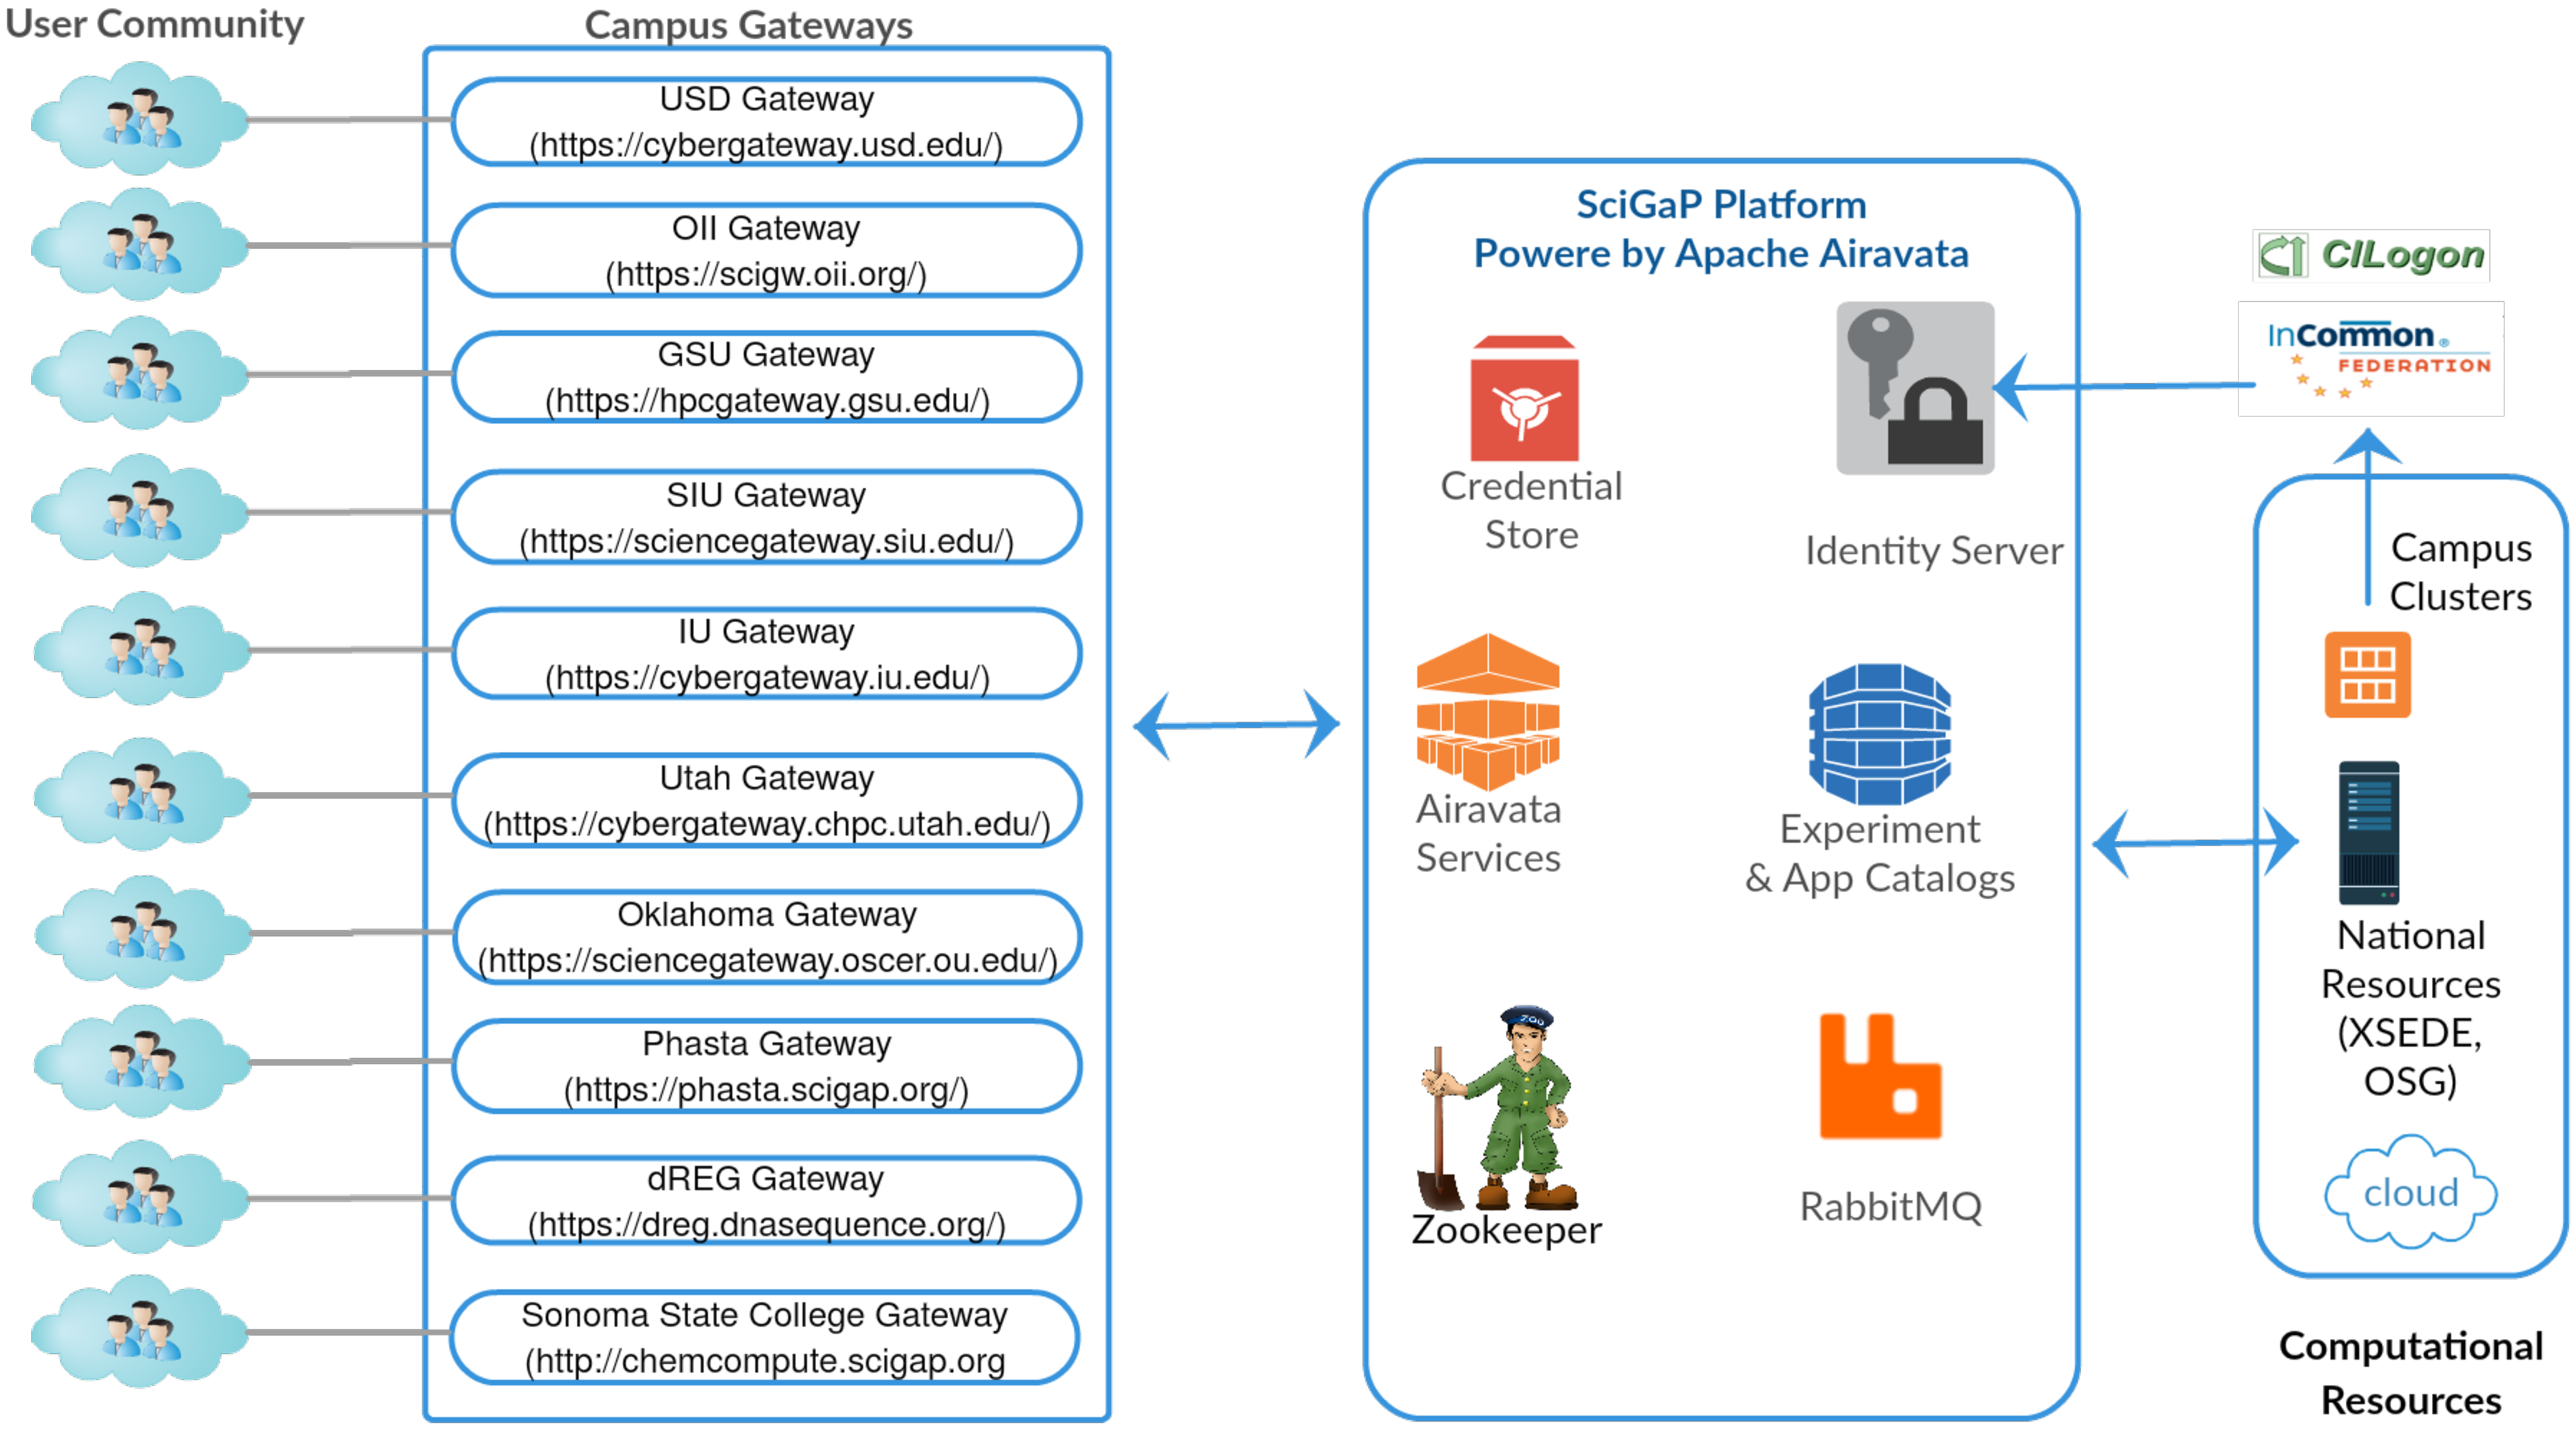
\includegraphics[height=4.5in, width=7in]{figures/gateway_deployments.pdf}
\caption{Science gateways with Airavata middleware and computational resources}
\end{figure*}

At the most basic level, hosting a gateway using an existing instance of multi-tenant supporting middleware is a two-step process: 1) deployment and 2) configuration.  However, in a university environment, there are situations that are going to add a layer of complexity to the installation. In order to host a gateway successfully we obtain the services from gateway providers, gateway administrators/PIs and cluster technical staff.  

Figure 1 illustrates a set of hosted gateways using Apache Airavata hosted middleware. One of the goals of the SciGaP project is to expand beyond our initial collaborating gateways (CIPRES, Neuroscience Gateway, and UltraScan) to provide a general purpose infrastructure.  The Identity Server \cite{nakandala2016apache} at the top of the figure provides authentication and authorization for Airavata and related SciGaP services shown in the middle box. 

When deploying these science gateways we identified three main categories:  general purpose gateways that need to support a diverse application set, domain-centric gateways that focus on a particular field of science, and application-centric gateways that focus on making a particular application or set of applications easier to use. Campus gateways fall into the general purpose category and are dedicated to a single campus and its collaborative research work. They may wish to offer up a very diverse set of applications.  Domain-centric gateways target  certain fields, but are more generic in providing applications to their users and are not tied to specific resources. That is, the gateway provider and the resource provider are distinct. In both cases, users will find a mixed combination of published and licensed applications, as well as privately developed applications and softwares. Finally, application centric gateways (such as PHASTA and dREG) focus on providing only a single application or set of closely related applications in order to increase the usability and adoption of a particular code. Like domain-specific gateways, application gateways are not tied to specific resources. 

Figure 2 illustrates the way a potential gateway administrator would go about requesting an Apache Airavata gateway through the SciGaP platform.  Requests are made through our SciGaP platform, and once received they are evaluated by our SciGaP team.  When the request is evaluated and  approved, gateway requested person  (typically the potential gateway administrator) is informed and together gateway is configured by providing gateway preferences, typical applications, storage resources, etc.  After this is completed, the initial group of users are invited to submit jobs through the gateway.  Although this sounds straightforward, there are consistent challenges we have faced as we have worked through this process with various institutions.  Below we share some of the most common challenges as well as some strategies we have adopted to face them. 

\begin{figure*}
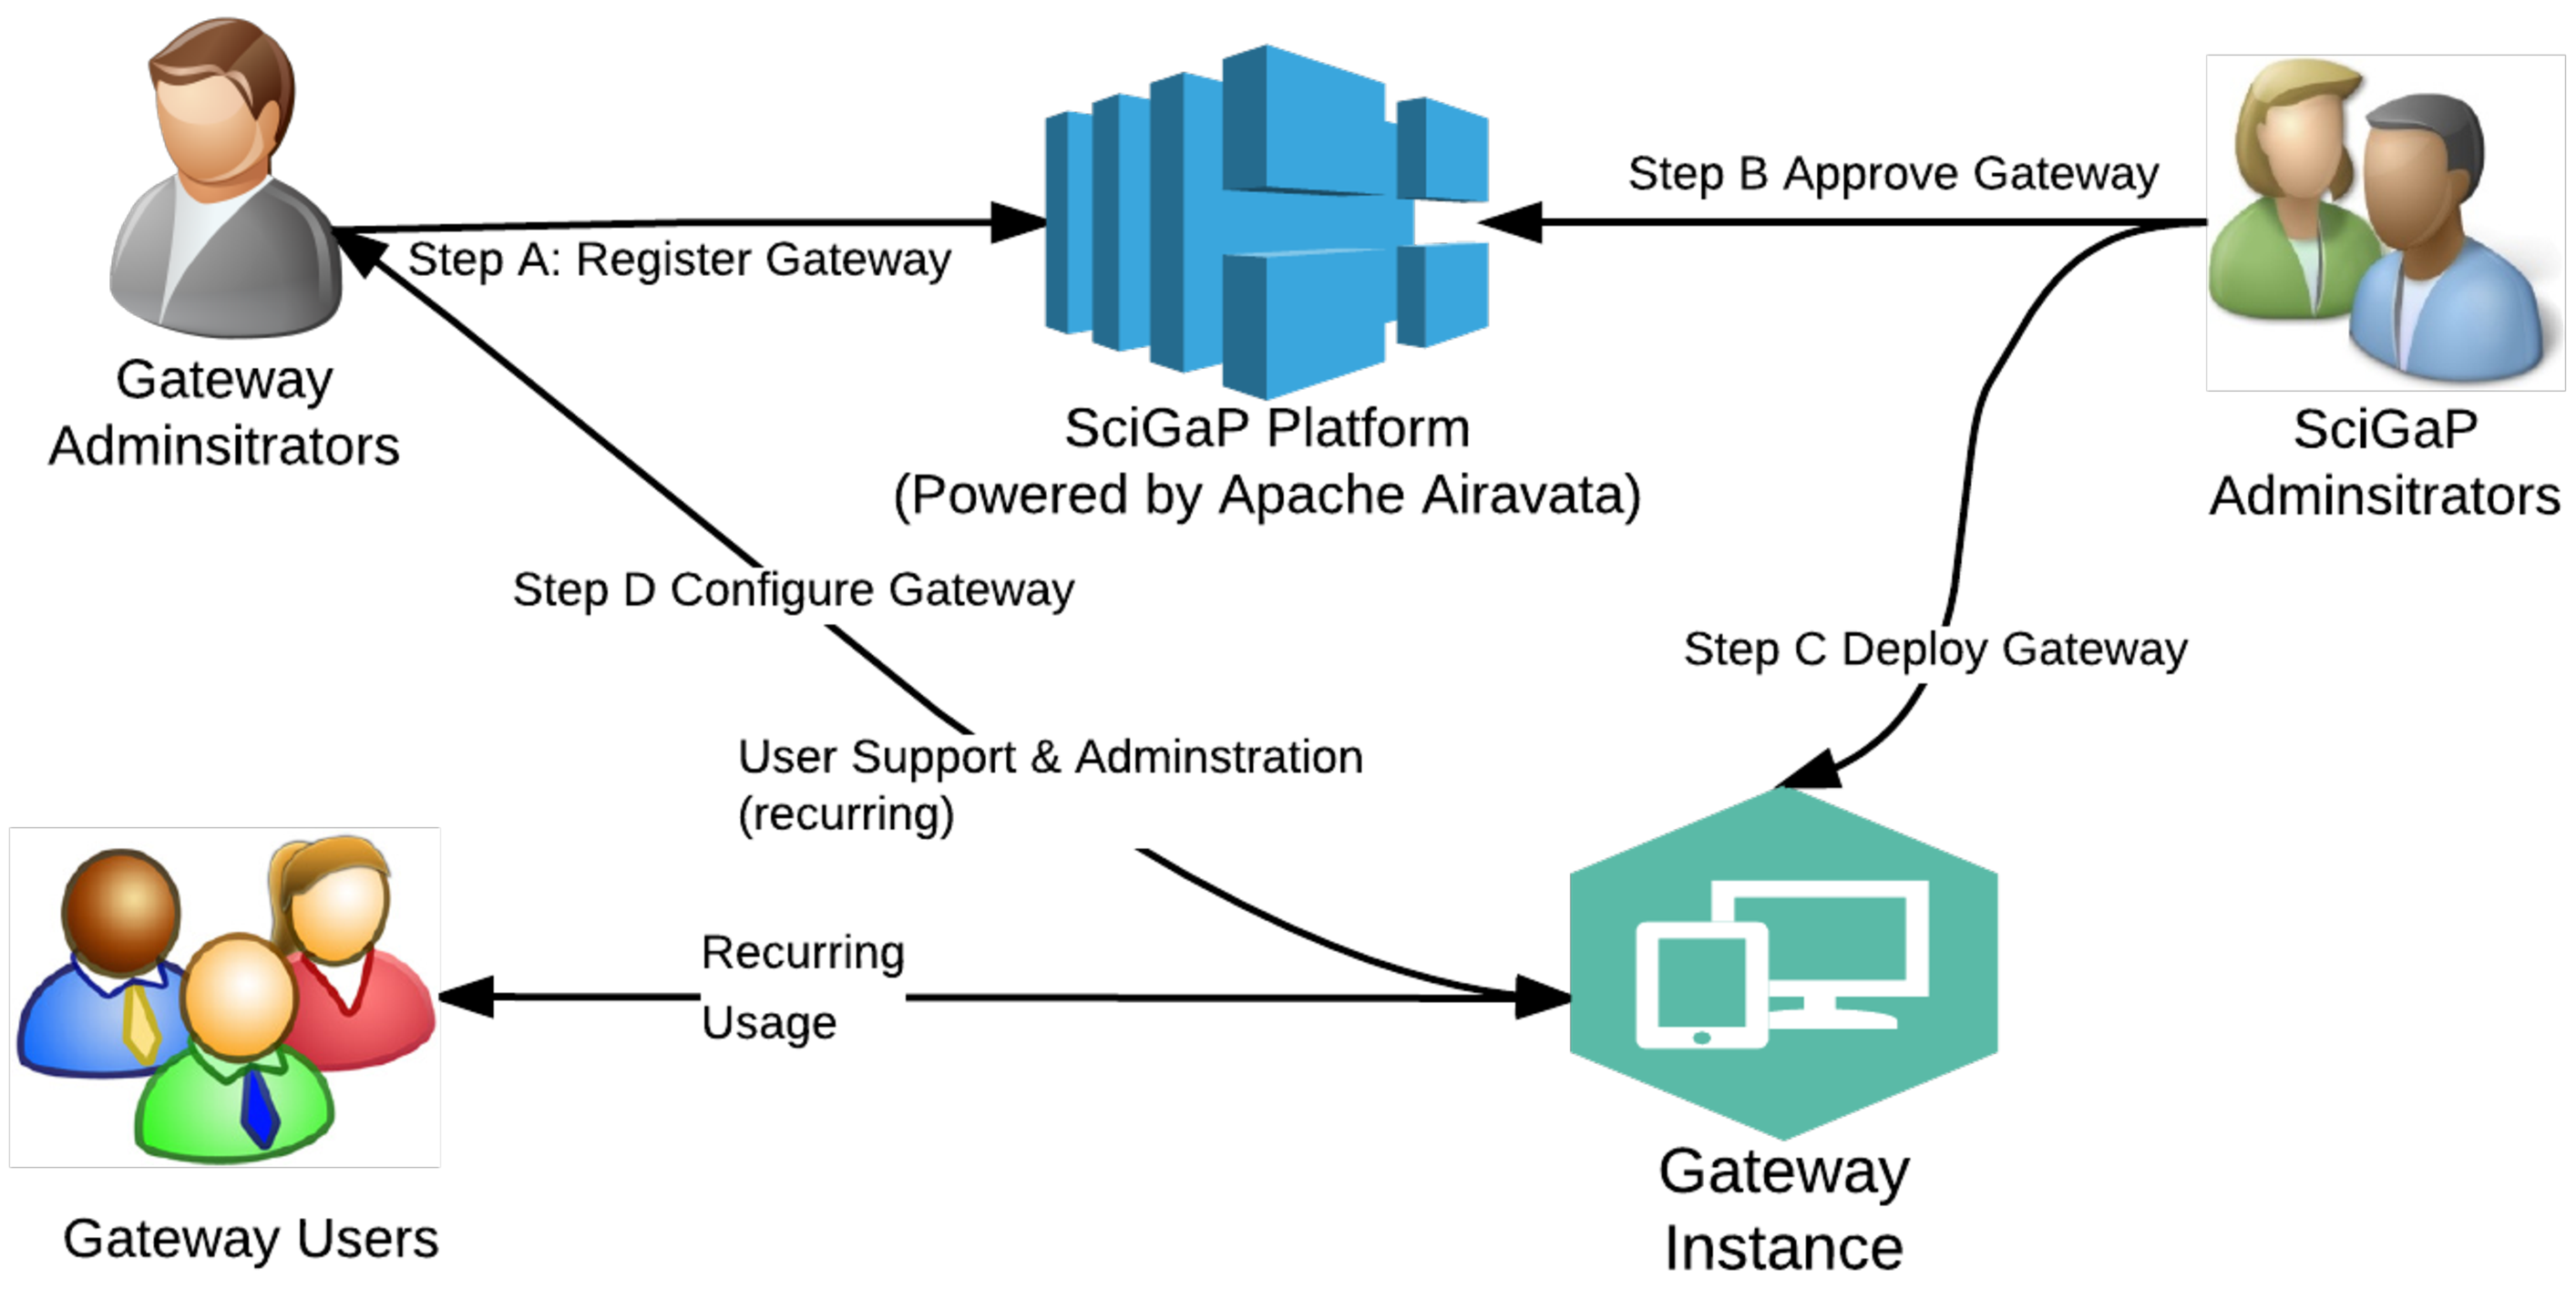
\includegraphics[height=3in, width=6in]{figures/gateway-approvals.pdf}
\caption{Workflow illustrating steps from requesting a gateway to using and providing support}
\end{figure*}

\section{Challenges Providing Campus Gateways}
As we extend the SciGaP platform services to include campus resources, we encountered several challenges described below.

\noindent\textbf{No Community Accounts}: Most of the institutions and campuses we have worked with have not wanted to distribute group or community accounts \cite{welch2007aaaa}. This is understandable given the need to account for computing resources, the need for security, and the possibility of audit. For this reason, we encourage users to use their own cluster allocation for job submissions. This leads to users having to take necessary steps to add their public keys to their cluster allocation, which in turn leads to more work for cluster administrators.  This is currently one of the primary issues we are working on. One solution involves automating the process of adding the public key to user allocation in the cluster.  For example,  when the user logs in to the gateway for the first time, a generated key will be added for ssh communications.

\noindent\textbf{Diverse User Management}: Campuses follow different protocols and mechanisms for user authentications. Gateway deployments for each of these campuses have to adapt to these diverse mechanisms. Gateway administrators also differ in defining policies for onboarding users onto a gateway.  Almost all campuses prefer to enable their campus identity systems to access the portal, thus avoiding a manual user management within the gateway. To meet these requirements, Airavata integrated with InCommon Federation and CILogon Identity brokering. Some campuses have LDAP servers dedicated to the research infrastructure and the gateway has to be integrated with these systems.  A few gateways prefer to maintain  a stand alone user management where users operate the gateway upon account validation (without administrative approval). These variations are enabled within Airavata using Industry standard security protocols and the use of Open Source Identity Servers. Airavata currently uses WSO2 Identity Server \cite{wso2IS} and is evaluating the feasibility of  migrating to Redhat's KeyClock Identity Server \cite{keycloak}.

\noindent\textbf{Legacy Systems}: While working with campus clusters we have encountered diverse job-schedulers and multiple versions of software applications. Clusters are designed to be refreshed every three years, but often they are not, and financial constraints and familiarity both contribute to the use of legacy software. In situations where older software versions are being run on an outdated infrastructure, technical issues with the gateway are going to occur.  Specifically, the lack of proper module commands forces significant collaboration between gateway consultants and gateway administrators. This challenge can only be mitigated through timely updates and proper maintenance of both software and hardware.  When gateway cluster-based issues arise,  technical support from someone familiar with the cluster is essential. Many science gateway clusters do not have a dedicated technical staff, and this complicates solving problems and increases wait times for doing so. It is expected that there is a gateway administrator who would champion the gateway from campus user support organizations ably supported by their own cluster technical staff. 

For gateways to enable job submissions to clusters, a programmatic way to monitor progress is required. Airavata currently relies on email-based monitoring as all job managers reliably send emails upon job status changes. In gateway clusters this is initially challenging because the email formats and the content are not automatically identified with the job status. Multiple rounds of testing need to be done in order to finalize email formats and content with correct job status updates. This requires time and energy from gateway providers, gateway administrators and cluster technical staff. In most cases the technical assistance also is provided by the gateway administrators. In the future we plan to explore alternative job monitoring mechanisms so it is  not required to solely rely on email-based monitoring systems. 

\noindent\textbf{Feature Support}: Apache Airavata is open source software to which anyone can contribute. Apache Airavata supports the integration of arbitrary gateways through its Application Programming Interface (API), which can be used by any gateway developer. We provide also a reference implementation, the PHP Gateway for Airavata (PGA), which can be simply taken and used with minimal theming. 

The key advantage of a centralized platform gateway is that it allows campus support staff to outsource their gateway operations. In our experience, campus gateway providers are less likely to want to make extensive customizations to their gateway when compared to application and domain-centric gateway providers. Campuses prefer to make requests for features and changes from the gateway providers.  When managing multiple gateways, gateway providers can end up with a pipeline of feature requests.  While this may result in delays from the gateway tenant's point of view, it does help us as platform providers to identify particularly important, cross-cutting features that need to be implemented. 

\section{Future Work}
First, we must reduce the number of human interactions needed to deploy a gateway. We are working to reduce the time for gateway deployment and configuration and to automate the process as much as possible. Second, at this time, campus clusters need to be added to the gateway by the SciGaP administrators.  In the future this will be a task for the gateway administrators themselves because we are actively assembling publicly-available resources  on deploying gateways and will soon have a catalogue of  working examples.  Third, we must unify the user provisioning process between the gateway and the cluster.  Currently this requires the manual step of adding public keys generated by the gateway to a user's authorized\_keys file in clusters. Fourth, the diversity of deployments of schedulers and resource managers on campuses has challenged our current solutions for generating queuing scripts because of the variety of applications and softwares deployed in various campus clusters. Currently, we generate individual solutions foreach new deployment; moving forward we intend to develop a more refined and more generic application property configuration.. Fifth, we need to revisit our permission models to make it easier for ``power'' users to have access to administrative methods in the API in order to control their deployments within a gateway. These operations are currently restricted to administrators. Gateway providers will have to decide who should have this privilege. 


\begin{acks}
We would like to thank Research Cyberinfrastructure administrators for their interest, support and commitment in deploying and operating science gateways at their respective institutions. Our thanks to Douglas Jennewein, University of South Dakota; Ryan Quinn, Oklahoma Innovation Institute; Semir Sarajlic, Georgia State University; Chester Langin, Southern Illinois University; Anita Orendt, University of Utah; Henry Neeman, University of Oklahoma; Cameron Smith, Phasta Gateway; Charles Danko, dREG Gateway and Mark Perri, Chemcompute Gateway. 

\end{acks}

\bibliographystyle{ACM-Reference-Format}
\bibliography{campus-gateways-pearc17}

\end{document}
